\documentclass[12pt,
aspectratio=169,
]{beamer} 

\setbeamersize{sidebar width right=0.1\paperwidth} 

\def \vkrtheme{Universidade Presbiteriana Mackenzie} 
\def \studentnumber{719535-90}
\def \studentfio{Brian Lee Mayer}
\def \rukovodfio{Luiz Henrique Alves Monteiro}

\def \imagedir{images/}
\def \libfile{vkr_lib.bib}

\usepackage{tex/PnuPresentStyle}

\begin{document}

\begin{titleframe}
	\begin{center}
		\includegraphics[width=2cm]{images/M_vermelho.pdf}\\[0.2cm]
		\begin{beamercolorbox}[sep=5pt,center]{title}
			\usebeamerfont{title}
			\insertsectionhead\par
			\inserttitle\par\insertsubtitle
		\end{beamercolorbox}
	\end{center}
	\insertsectionhead\par
		\large \bf\insertauthor\\
	\vfill
	\begin{center}\large \bf\insertdate\end{center}
\end{titleframe}

\begin{frame}
\frametitle{\'Indice}
\tableofcontents
\end{frame}

\section{Introdução}

\begin{frame}{Introdução}
Defini\c c\~ao: Um $d$-primo \'e um n\'umero natural que possui exatamente $d$ divisores.

Utiliza-se a nota\c c\~ao $p_d(x)$ para denotar o $x$-\'esimo n\'umero com $d$ divisores.

\end{frame}

\begin{frame}{Introdução}
Assim classificamos os n\'umeros pelos seus divisores:

\begin{tabular}{|c|l|} \hline
        $d$ & $p_d(n)$ \\
        \hline
        2 & $2, 3, 5, 7, 11, 13, 17, 19, 23, 29, 31, 37, 41, \ldots$ \\
        3 & $4, 9, 25, 49, 121, 169, 289, 361, 529, 841, \ldots$ \\
        % 4 & $6, 8, 10, 14, 15, 21, 22, 26, 27, 33, 34, 35, \ldots$ \\
        % 5 & $16, 81, 625, 2401, 14641, 28561, 83521, \ldots$ \\
        % 6 & $12, 18, 20, 28, 32, 44, 45, 50, 52, 63, 68, 75 \ldots$ \\
        % 7 & $64, 729, 15625, 117649, 1771561, 4826809, \ldots$ \\
        % 8 & $24, 30, 40, 42, 54, 56, 66, 70, 78, 88, 102, \ldots$ \\
        % 9 & $36, 100, 196, 225, 256, 441, 484, 676, 1089, \ldots$ \\
        % 10 & $48, 80, 112, 162, 176, 208, 272, 304, 368, \ldots$ \\
        & \\
        \vdots & \vdots \\
        & \\
        % 11 & $ 1024, 59049, 9765625, 282475249, \ldots$ \\
        12 & $ 60, 72, 84, 90, 96, 108, 126, 132, 140, 150, \ldots$ \\
        13 & $ 4096, 531441, 244140625, 13841287201, \ldots$ \\
        14 & $ 192, 320, 448, 704, 832, 1088, 1216, 1458, \ldots$ \\
        15 & $ 16384, 4782969, 6103515625, 678223072849, \ldots$ \\
        16 & $120, 168, 210, 216, 264, 270, 280, 312, 330, \ldots$ \\
        \hline
    \end{tabular}
    \label{tab:n-primes}
\end{frame}


\begin{frame}{Introdução}

O maior número utilizado nesta tese é o $p_{13}(10000)$ cujo valor é:
$$1741018879299188426700762715443778414040036179271771734964641$$

Esse número possui 61 dígitos, e 61 é, curiosamente, um número 2-primo.[[]]
\end{frame}


\begin{frame}{Algoritmo de Visibilidade Natural}
\paragraph{Método:} Sejam $a$, $b$ e $i$ indices de uma sequência
$x(n)$, com  $a < i < b$. No grafo de visibilidade
natural (VN), $x(a)$ e $x(b)$ estão conectados se todos os pontos
intermediários $(i, x(i))$ satisfazem a desigualdade:
\begin{equation}
\label{nv}
x(i) < x(a) + \left( x(b)-x(a) \right) \left(
\frac{i - a}{b-a} \right)
\end{equation}

\begin{tabular}{c c c}
      \includegraphics[width=0.4\textwidth]{images/example-plot-natural.pdf} & $\to$
     & \includegraphics[width=0.4\textwidth]{images/example-graph-natural.pdf} \\
\end{tabular}
   
\end{frame}


\begin{frame}{Algoritmo de Visibilidade Horizontal}
No grafo de visibilidade horizontal (VH), os nós
$x(a)$ e $x(b)$ estão conectados se
todos os pontos intermediários $(i,x(i))$ no gráfico $x(n) \times
n$ estão abaixo da linha horizontal que une  $(a, x(a))$ e
$(b,x(b))$. 

\begin{tabular}{c c c}
      \includegraphics[width=0.4\textwidth]{images/example-plot-horizontal.pdf} & $\to$
     & \includegraphics[width=0.4\textwidth]{images/example-graph-horizontal.pdf} \\
\end{tabular}
   
\end{frame}

\begin{frame}{Estudos}
Estudos com $d$-primos:
\begin{itemize}
    \item Visibilidades das lacunas
    \item Densidade
    \item Grafos de divisores e orbitas
    \item Complexidade SDL
\end{itemize}

\vspace{10pt}
Estudos com divisores de n\'umeros naturais e felizes:
\begin{itemize}
    \item Visibilidades das casas decimais
    \item Visibilidades de duplas de casas decimais
    \item Visibilidades de triplas de casas decimais
    \item Complexidade SDL
\end{itemize}
\end{frame}


\section{Resultados}

\begin{nobarframe}
\vfill
\begin{center}
\Large
Resultados
\end{center}
\vfill
\end{nobarframe}

\begin{frame}{Lacunas de $d$-primos}
    
\begin{table}[ht]
\begin{center}
\caption{Entropia informacional normalizada $h$ de $x_d(n)$ para
$d \in \{2, 3, \ldots, 11\}$.}
\small
\begin{tabular}{|c|c|c|c|c|c|c|c|c|c|c|} \hline
        $d$ & 2 & 3 & 4 & 5 & 6 & 7 & 8 & 9 & 10 & 11\\ \hline
        $h$ & 0.713 & 0.997 & 0.653 & 1 & 0.797 & 1 & 0.696 &
        0.999 & 0.700 & 1\\
        \hline
    \end{tabular}
    \label{entropies}
\end{center}
\end{table}
\end{frame}


\subsection{Visibilidades das lacunas}
\begin{nobarframe}

\begin{table}[h!]
\begin{center}
\caption{Valores de $A$ e $\gamma$ correspondentes ao ajuste da distribuição de graus
$P(k)=A k^{-\gamma}$ e o grau médio $\langle k \rangle $ em função de $d$
para os grafos de VN.}
\begin{tabular}{|c|c|c|c|c|c|c|}\hline
        visibilidade & $d$ & $A$ & $\gamma$  & $\langle k \rangle $ \\
        \hline
        natural & 2 & $0.4 \pm 0.1$  & $1.1 \pm 0.2$ & 6.17 \\
        natural & 3 & $0.4 \pm 0.1$  & $1.1 \pm 0.2$ & 6.52 \\
        natural & 4 & $1.2 \pm 0.2$  & $1.6 \pm 0.1$ & 6.40 \\
        natural & 5 & $1.03 \pm 0.07$ & $1.53 \pm 0.05$ & 14.3 \\
        natural & 6 & $0.5 \pm 0.1$ & $1.1 \pm 0.2$ & 6.33 \\
natural & 7 & $0.29 \pm 0.03$ & $1.02 \pm 0.06$ & 27.7 \\
natural & 8 & $0.4 \pm 0.1$ & $1.1 \pm 0.2$ & 6.28 \\
natural & 9 & $0.12 \pm 0.05$ & $0.6 \pm 0.2$ & 6.66 \\
natural & 10 & $0.4 \pm 0.1$ & $1.1 \pm 0.2$ & 6.23 \\
natural & 11 & $0.19 \pm 0.02$ & $0.91 \pm 0.04$ & 45.2 \\
        \hline
    \end{tabular}
    \label{tab:natural-stats}
\end{center}
\end{table}
\end{nobarframe}


\begin{nobarframe}

\begin{table}[H]
\begin{center}
\caption{Valores de $A$ e $\gamma$ correspondentes ao ajuste da distribuição de graus
$P(k)=A k^{-\gamma}$ e o grau médio $\langle k \rangle $ em função de $d$
para os grafos de VH.}
\begin{tabular}{|c|c|c|c|c|c|c|}\hline
        visibilidade & $d$ & $A$ & $\gamma$  & $\langle k \rangle $ \\
        \hline
horizontal & 2 & $1.2 \pm 0.3$  & $1.7 \pm 0.3$ & 3.67 \\
horizontal & 3 & $1.1 \pm 0.2$  & $1.6 \pm 0.2$ & 3.98 \\
horizontal & 4 & $1.7 \pm 0.2$  & $1.9 \pm 0.2$ & 3.47 \\
horizontal & 5 & $1.1 \pm 0.2$  & $1.6 \pm 0.2$ & 3.97 \\
horizontal & 6 & $1.1 \pm 0.2$  & $1.6 \pm 0.2$ & 3.89 \\
horizontal & 7 & $1.1 \pm 0.2$  & $1.6 \pm 0.2$ & 3.96 \\
horizontal & 8 & $1.5 \pm 0.2$  & $1.8 \pm 0.2$ & 3.59 \\
horizontal & 9 & $1.0 \pm 0.2$  & $1.6 \pm 0.2$ & 3.99 \\
horizontal & 10 & $1.1 \pm 0.2$ & $1.6 \pm 0.2$ & 3.84 \\
horizontal & 11 & $1.1 \pm 0.2$ & $1.6 \pm 0.2$ & 3.95 \\
        \hline
    \end{tabular}
    \label{tab:horizontal-stats}
\end{center}
\end{table}
\end{nobarframe}


\subsection{Sequ\^encias de divisores}
\begin{frame}{Sequ\^encias de divisores}

\begin{figure}[H]
    \centering
    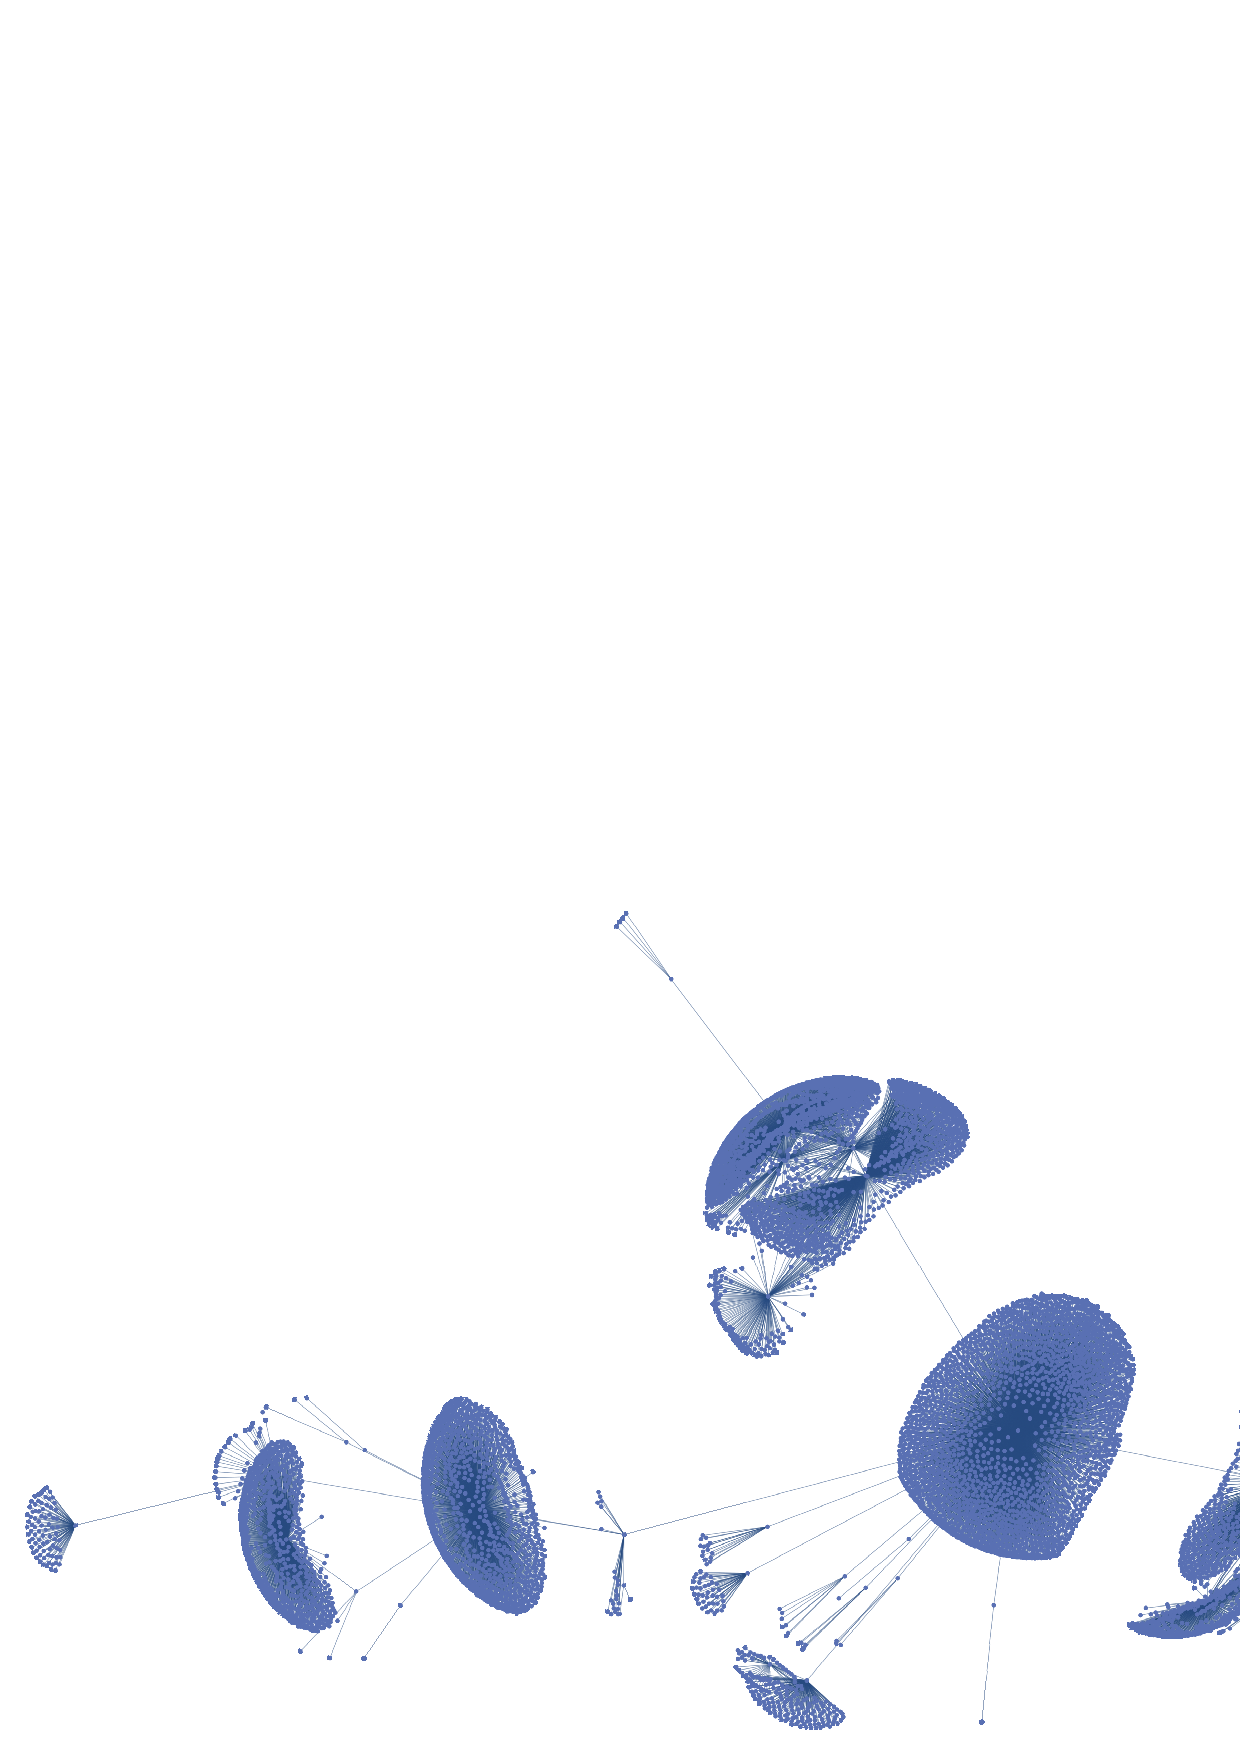
\includegraphics[width=0.6\textwidth]{images/divisors.pdf}
    \caption{As ligações são estabelecidas entre um número
    e sua quantidade de divisores.}
    \label{graph-divs}
\end{figure}
\end{frame}


\begin{frame}{Sequ\^encias de divisores}
\begin{figure}[H]
    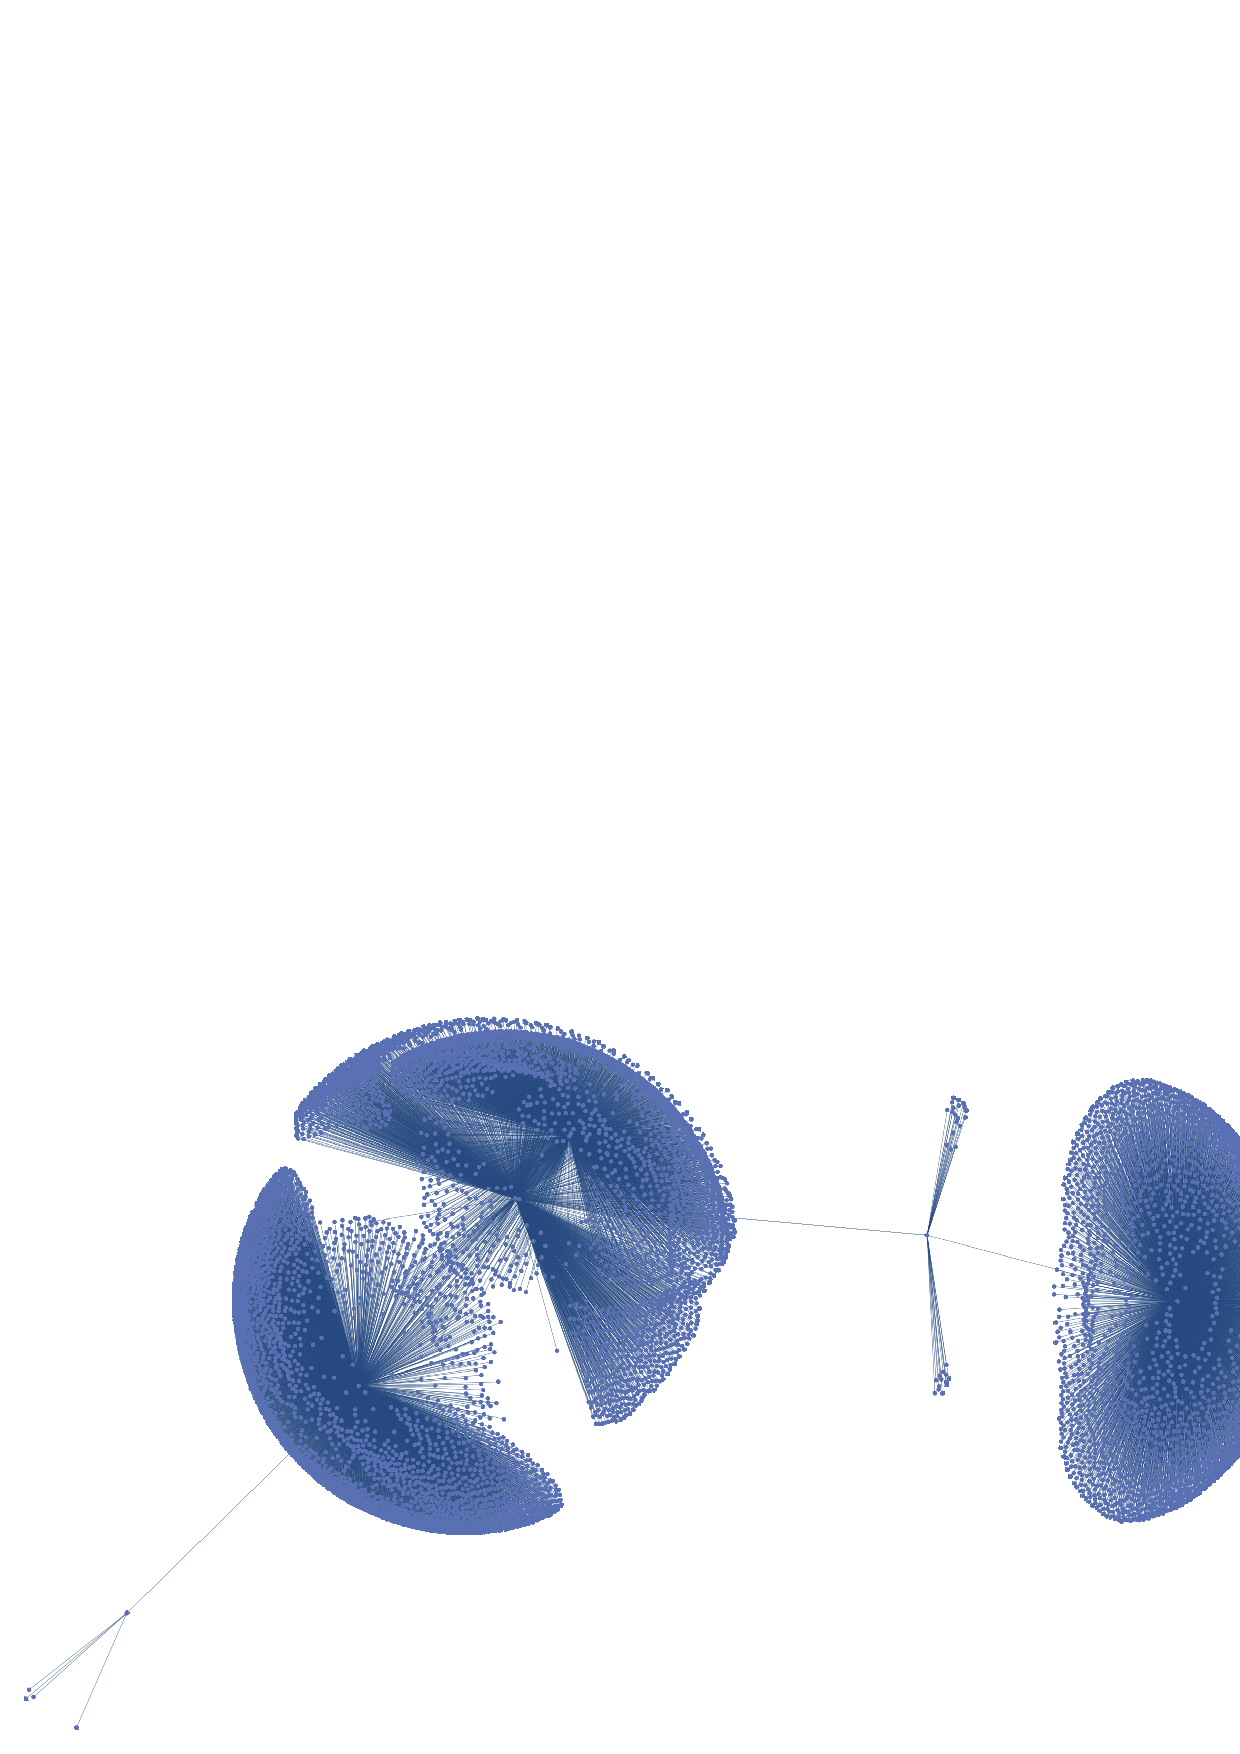
\includegraphics[width=0.65\textwidth]{images/orbits.pdf}
    \centering
    \caption{\centering As ligações são estabelecidas entre um número
    e sua quantidade de divisores.}
    \label{graph-divs}
\end{figure}
\end{frame}


\begin{nobarframe}
    
\begin{table}[H]
    \caption{\centering Valores de $A$ e $\gamma$ para os grafos de VH e VN.}
    \begin{tabular}{|c|c|c|c|c|}
        \hline série & visibilidade & $\langle k \rangle$ & $\gamma$ & $A$ \\
        \hline
        divisores & natural & 5.6 & $1.2 \pm 0.2$ & $0.56 \pm 0.13$ \\
        divisores & horizontal & 3.6 & $0.64 \pm 0.66$ & $0.19 \pm 0.17$ \\
        órbitas & natural & 4.9 & $0.56 \pm 0.41$ & $0.15 \pm 0.10$ \\
        órbitas & horizontal & 3.0 & $0.3 \pm 1.6$ & $0.20 \pm 0.39$ \\
         \hline 
    \end{tabular}
    \label{tab:div-orb}
\end{table}

\end{nobarframe}
\subsection{Densidades}
\begin{frame}{Densidade}
\begin{itemize}
    \item Nota-se que existe uma distin\c c\~ao de comportamento na densidade dos d-primos entre $d$ par e \'\i mpar.
    \item  Dentre os pares, apenas para $d = 8$ a densidade tem concavidade voltada para baixo; para as demais curvas com $d$ par, a densidade tem concavidade voltada para cima.
    \item Esse comportamento tamb\'em pode se repetir para valores maiores de $d$, com mais estudos poderemos conjecturar a depend\^encia da densidade entre os valores de $d$, em especial, com a densidade para $d = 2$.
\end{itemize}
\end{frame}


\subsection{D\'\i gitos de n\'umeros irracionais}


\begin{frame}{N\'umeros irracionais}

\begin{itemize}
    \item Os histogramas aproximadamente constantes sugerem aleatoriedade uniforme
    \item Os valores de $\langle k \rangle$, A e $\gamma$ s\~ao muito pr\'oximos para todos os grafos. Pode-se conjecturar que os dois algoritmos de visibilidade n\~ao diferenciam n\'umeros transcendentais dos irracionais. 
\end{itemize}
\end{frame}


\begin{nobarframe}

\begin{table}[H]
    \small
    \caption{ Propriedades dos grafos gerados a partir de números irracionais.}
    \begin{tabular}{|c|cc|ccc|ccc|}
    \hline
 &&& \multicolumn{3}{|c|}{Visibilidade Natural} & \multicolumn{3}{|c|}{Visibilidade Horizontal} \\
& $C_{SDL}$ & $h$ & $\langle k \rangle$ & $A$ & $\gamma$  & $\langle k \rangle$ & $A$ & $\gamma$ \\
\hline 
 $\sqrt{2}$     & 0.194 & 0.948 & 5.19 & 0.70$\pm$0.13 & 1.34$\pm$0.16 & 3.63 & 1.33$\pm$0.26 & 1.73$\pm$0.20 \\
 $\sqrt{2}_2$   & 0.135 & 0.964 & 5.40 & 0.65$\pm$0.12 & 1.30$\pm$0.15 & 3.95 & 1.21$\pm$0.17 & 1.69$\pm$0.14 \\
 $\sqrt{2}_3$   & 0.097 & 0.975 & 5.39 & 0.66$\pm$0.12 & 1.31$\pm$0.15 & 3.99 & 1.21$\pm$0.16 & 1.69$\pm$0.13 \\
 $\phi$         & 0.192 & 0.949 & 5.21 & 0.69$\pm$0.13 & 1.33$\pm$0.17 & 3.63 & 1.32$\pm$0.26 & 1.73$\pm$0.21 \\
 $\phi_2$       & 0.136 & 0.964 & 5.37 & 0.66$\pm$0.12 & 1.31$\pm$0.15 & 3.95 & 1.22$\pm$0.17 & 1.69$\pm$0.15 \\
 $\phi_3$       & 0.096 & 0.975 & 5.37 & 0.66$\pm$0.13 & 1.31$\pm$0.16 & 3.99 & 1.20$\pm$0.17 & 1.68$\pm$0.14 \\
 $e$            & 0.195 & 0.948 & 5.21 & 0.69$\pm$0.13 & 1.33$\pm$0.16 & 3.64 & 1.33$\pm$0.24 & 1.73$\pm$0.19 \\
 $e_2$          & 0.149 & 0.961 & 5.35 & 0.65$\pm$0.13 & 1.30$\pm$0.16 & 3.94 & 1.22$\pm$0.17 & 1.69$\pm$0.14 \\
 $e_3$          & 0.096 & 0.975 & 5.35 & 0.67$\pm$0.12 & 1.32$\pm$0.15 & 3.99 & 1.22$\pm$0.15 & 1.69$\pm$0.13 \\
 $\pi$          & 0.192 & 0.949 & 5.19 & 0.70$\pm$0.13 & 1.34$\pm$0.16 & 3.64 & 1.33$\pm$0.25 & 1.73$\pm$0.19 \\
 $\pi_2$        & 0.145 & 0.962 & 5.38 & 0.65$\pm$0.12 & 1.30$\pm$0.16 & 3.95 & 1.21$\pm$0.17 & 1.68$\pm$0.14 \\
 $\pi_3$        & 0.100 & 0.974 & 5.37 & 0.66$\pm$0.14 & 1.31$\pm$0.15 & 3.99 & 1.20$\pm$0.17 & 1.68$\pm$0.15 \\
 \hline
\end{tabular}
    \label{tab:numbers}
\end{table}
\end{nobarframe}


\section{Conclusão}


\begin{nobarframe}
\vfill
\begin{center}
\Large
Conclusão
\end{center}
\vfill
\end{nobarframe}


\begin{frame}{Lacunas entre $d$-primos}
    \begin{itemize}
        \item Os grafos das sequ\^encias de $d$-primos possuem $P(k) = A k−\gamma$; 
        ou seja, $P(k)$ segue uma lei de pot\^encia.  Portanto, esses
grafos s\~ao livres de escala. Implicando autossimilaridade.

    \item $h$, a entropia normalizada, distingue $d$ par dos \'\i mpares. 
    \item $\langle k \rangle$ distingue $d$ primos dos
$d$ n\~ao  primos para a VN;
    \item Artigo publicado: \emph{A Numerical Study on the Regularity of d-Primes via Informational Entropy and Visibility Algorithms}
    \end{itemize}
\end{frame}


\begin{frame}{Densidades de $d$-primos}
    \begin{itemize}
        \item Apenas para $d = 8$ a densidade tem concavidade voltada para baixo.
        \item Em todos os casos a converg\^encia \'e semelhante a do caso usual dos primos, i.e. $d=2$.
    \end{itemize}
\end{frame}


\begin{frame}{Sequ\^encias de divisores e \'orbitas}
    \begin{itemize}
        \item A sequ\^encia de divisores e a sequ\^encia das \'orbitas dos divisores levaram a grafos de VN e VH em que $P(k) = A k−\gamma$; ou seja, $P(k)$ segue uma lei de pot\^encia. Portanto, esses
grafos s\~ao livres de escala. 
        \item Al\'em disso, o coeficiente $\gamma$ para a sequ\^encia das \'orbitas \'e aproximadamente metade daquele relacionado \`a sequ\^encia dos divisores.
        
    \end{itemize}
\end{frame}


\section{Trabalhos futuros}
\begin{frame}{Trabalhos futuros}
    \begin{itemize}
        \item Considerar sequ\^encias maiores
        \item Iniciar estudo com fra\c c\~oes cont\'\i nuas
        \item Determinar valores das converg\^encias das densidades
        \item Verificar rela\c c\~ao entre os resultados das visibilidades e o valor das lacunas
        \item Usar mais valores de $d$ nos $d$-primos
    \end{itemize}
\end{frame}


% \section{Refer\^encias} % Not belong to any section

% \begin{frame}
% %	[allowframebreaks]
% \frametitle{Refer\^encias}
% % \usebeamercolor{normal text}
% \printbibliography[heading=bibintoc]
% \end{frame}


\begin{nobarframe}
\vfill
\begin{center}
\Large
Obrigado!
\end{center}
\vfill
\end{nobarframe}

\end{document}
